% Options for packages loaded elsewhere
% Options for packages loaded elsewhere
\PassOptionsToPackage{unicode}{hyperref}
\PassOptionsToPackage{hyphens}{url}
%
\documentclass[
  ignorenonframetext,
  aspectratio=169,
]{beamer}
\newif\ifbibliography
\usepackage{pgfpages}
\setbeamertemplate{caption}[numbered]
\setbeamertemplate{caption label separator}{: }
\setbeamercolor{caption name}{fg=normal text.fg}
\beamertemplatenavigationsymbolsempty
% remove section numbering
\setbeamertemplate{part page}{
  \centering
  \begin{beamercolorbox}[sep=16pt,center]{part title}
    \usebeamerfont{part title}\insertpart\par
  \end{beamercolorbox}
}
\setbeamertemplate{section page}{
  \centering
  \begin{beamercolorbox}[sep=12pt,center]{section title}
    \usebeamerfont{section title}\insertsection\par
  \end{beamercolorbox}
}
\setbeamertemplate{subsection page}{
  \centering
  \begin{beamercolorbox}[sep=8pt,center]{subsection title}
    \usebeamerfont{subsection title}\insertsubsection\par
  \end{beamercolorbox}
}
% Prevent slide breaks in the middle of a paragraph
\widowpenalties 1 10000
\raggedbottom
\AtBeginPart{
  \frame{\partpage}
}
\AtBeginSection{
  \ifbibliography
  \else
    \frame{\sectionpage}
  \fi
}
\AtBeginSubsection{
  \frame{\subsectionpage}
}
\usepackage{iftex}
\ifPDFTeX
  \usepackage[T1]{fontenc}
  \usepackage[utf8]{inputenc}
  \usepackage{textcomp} % provide euro and other symbols
\else % if luatex or xetex
  \usepackage{unicode-math} % this also loads fontspec
  \defaultfontfeatures{Scale=MatchLowercase}
  \defaultfontfeatures[\rmfamily]{Ligatures=TeX,Scale=1}
\fi
\usepackage{lmodern}

\ifPDFTeX\else
  % xetex/luatex font selection
\fi
% Use upquote if available, for straight quotes in verbatim environments
\IfFileExists{upquote.sty}{\usepackage{upquote}}{}
\IfFileExists{microtype.sty}{% use microtype if available
  \usepackage[]{microtype}
  \UseMicrotypeSet[protrusion]{basicmath} % disable protrusion for tt fonts
}{}
\makeatletter
\@ifundefined{KOMAClassName}{% if non-KOMA class
  \IfFileExists{parskip.sty}{%
    \usepackage{parskip}
  }{% else
    \setlength{\parindent}{0pt}
    \setlength{\parskip}{6pt plus 2pt minus 1pt}}
}{% if KOMA class
  \KOMAoptions{parskip=half}}
\makeatother


\usepackage{longtable,booktabs,array}
\newcounter{none} % for unnumbered tables
\usepackage{calc} % for calculating minipage widths
\usepackage{caption}
% Make caption package work with longtable
\makeatletter
\def\fnum@table{\tablename~\thetable}
\makeatother
\usepackage{graphicx}
\makeatletter
\newsavebox\pandoc@box
\newcommand*\pandocbounded[1]{% scales image to fit in text height/width
  \sbox\pandoc@box{#1}%
  \Gscale@div\@tempa{\textheight}{\dimexpr\ht\pandoc@box+\dp\pandoc@box\relax}%
  \Gscale@div\@tempb{\linewidth}{\wd\pandoc@box}%
  \ifdim\@tempb\p@<\@tempa\p@\let\@tempa\@tempb\fi% select the smaller of both
  \ifdim\@tempa\p@<\p@\scalebox{\@tempa}{\usebox\pandoc@box}%
  \else\usebox{\pandoc@box}%
  \fi%
}
% Set default figure placement to htbp
\def\fps@figure{htbp}
\makeatother





\setlength{\emergencystretch}{3em} % prevent overfull lines

\providecommand{\tightlist}{%
  \setlength{\itemsep}{0pt}\setlength{\parskip}{0pt}}



 


\setbeamertemplate{frametitle continuation}{} %to remove number after "Table of contents"
\setbeamertemplate{itemize items}[circle] %for itemize to be small circles
\usepackage{caption}
\captionsetup{labelformat=empty, justification=centering} %to remove "Figure X:" in captions and center txt
\usepackage{textpos} %for positioning image on top of everything
\setlength{\TPHorizModule}{1cm} %for positioning image on top of everything
\setlength{\TPVertModule}{1cm} %for positioning image on top of everything
\setbeamertemplate{footline}{%to count slides
  \hfill\usebeamercolor[fg]{page number in head/foot}%
  \usebeamerfont{page number in head/foot}%
  \insertframenumber{} / \inserttotalframenumber\kern1em\vskip2pt%
}
\makeatletter
\@ifpackageloaded{caption}{}{\usepackage{caption}}
\AtBeginDocument{%
\ifdefined\contentsname
  \renewcommand*\contentsname{Table of contents}
\else
  \newcommand\contentsname{Table of contents}
\fi
\ifdefined\listfigurename
  \renewcommand*\listfigurename{List of Figures}
\else
  \newcommand\listfigurename{List of Figures}
\fi
\ifdefined\listtablename
  \renewcommand*\listtablename{List of Tables}
\else
  \newcommand\listtablename{List of Tables}
\fi
\ifdefined\figurename
  \renewcommand*\figurename{Figure}
\else
  \newcommand\figurename{Figure}
\fi
\ifdefined\tablename
  \renewcommand*\tablename{Table}
\else
  \newcommand\tablename{Table}
\fi
}
\@ifpackageloaded{float}{}{\usepackage{float}}
\floatstyle{ruled}
\@ifundefined{c@chapter}{\newfloat{codelisting}{h}{lop}}{\newfloat{codelisting}{h}{lop}[chapter]}
\floatname{codelisting}{Listing}
\newcommand*\listoflistings{\listof{codelisting}{List of Listings}}
\makeatother
\makeatletter
\makeatother
\makeatletter
\@ifpackageloaded{caption}{}{\usepackage{caption}}
\@ifpackageloaded{subcaption}{}{\usepackage{subcaption}}
\makeatother

\usepackage{bookmark}
\IfFileExists{xurl.sty}{\usepackage{xurl}}{} % add URL line breaks if available
\urlstyle{same}
% fallback for those not using the hyperref driver hyperxmp:
\makeatletter
\@ifundefined{xmpquote}{\newcommand{\xmpquote}[1]{#1}}{}
\makeatother
\hypersetup{
  pdftitle={Introduction to Basic and Advanced Statistical Modelling},
  pdfauthor={Alexandre Courtiol},
  hidelinks,
  pdfcreator={LaTeX via pandoc}}


\title{\texorpdfstring{Introduction to Basic and Advanced Statistical
Modelling}{Introduction to Basic and Advanced Statistical Modelling}}
\subtitle{\texorpdfstring{Introduction}{Introduction}}
\author{Alexandre Courtiol}
\date{}

\begin{document}
\frame{\titlepage}

\renewcommand*\contentsname{Table of contents}
\begin{frame}[allowframebreaks]
  \frametitle{Table of contents}
  \setcounter{tocdepth}{3}
  \tableofcontents
\end{frame}
\setcounter{tocdepth}{3}
\tableofcontents
}

\section{About this workshop}\label{about-this-workshop}

\begin{frame}{Why this workshop?}
\protect\phantomsection\label{why-this-workshop}
\begin{itemize}[<+->]
\tightlist
\item
  Many local actors collect invaluable data on biodiversity in one of
  the most biodiversity-rich regions in the world
\item
  Much of these data remain unexploited and yet they could benefit both
  local conservation and the global scientific community
\item
  We believe one reason is that many local actors have limited
  quantitative skills
\item
  This workshop aims at strengthening local capacity by training local
  actors
\end{itemize}
\end{frame}

\begin{frame}{The workshop structure}
\protect\phantomsection\label{the-workshop-structure}
\begin{block}{Module A: background knowledge to prepare for Module B}
\protect\phantomsection\label{module-a-background-knowledge-to-prepare-for-module-b}
\begin{itemize}
\tightlist
\item
  foundation of the R language
\item
  introduction to reproducible reporting workflows
\item
  review of core statistical concepts
\item
  introduction to Linear Models (LMs, GLMs)
\end{itemize}

\pause
\end{block}

\begin{block}{Module B: applied methods}
\protect\phantomsection\label{module-b-applied-methods}
\begin{itemize}
\tightlist
\item
  single-species occupancy models
\item
  community-level frameworks
\item
  predicting and mapping occurrence and richness across the study area
\end{itemize}
\end{block}
\end{frame}

\section{About me, you \& us}\label{about-me-you-us}

\begin{frame}{The lecturers}
\protect\phantomsection\label{the-lecturers}
\begin{columns}[T]
\begin{column}{0.5\linewidth}
\centering

\textbf{Module A}: Alexandre Courtiol\\

\begin{center}
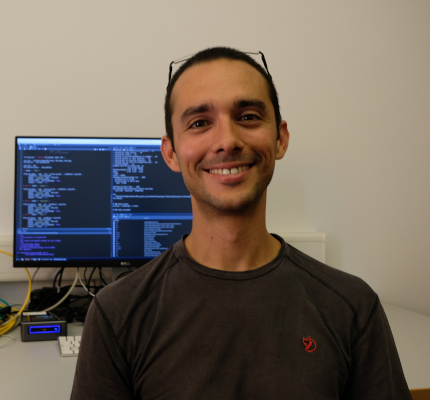
\includegraphics[width=\linewidth,height=5cm,keepaspectratio]{figures/Alexandre_Courtiol.jpg}
\end{center}
\end{column}

\begin{column}{0.5\linewidth}
\centering

\textbf{Module B}: Rahel Sollmann\\

\begin{center}
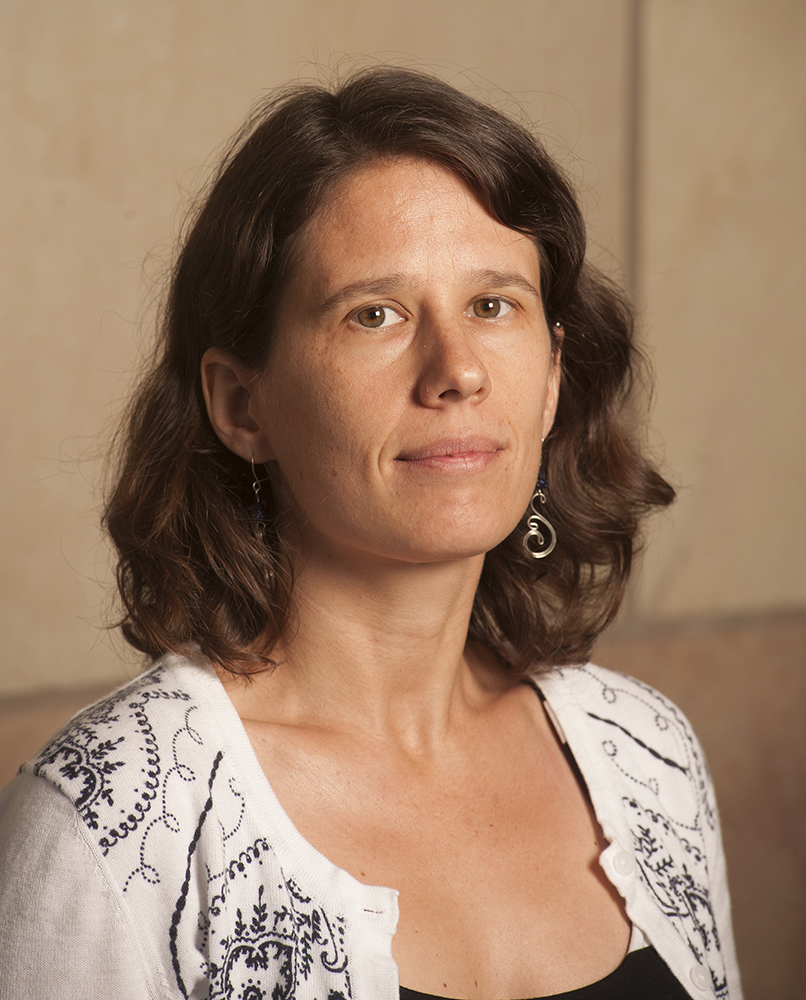
\includegraphics[width=\linewidth,height=5cm,keepaspectratio]{figures/Rahel_Sollmann.jpg}
\end{center}
\end{column}
\end{columns}
\end{frame}

\begin{frame}{Who am I?}
\protect\phantomsection\label{who-am-i}
\begin{block}{Quantitative population biologist}
\protect\phantomsection\label{quantitative-population-biologist}
\begin{itemize}[<+->]
\tightlist
\item
  trained in evolution, ecology, demography and statistics
\item
  leader of a small research team tackling diverse questions about the
  life history and behaviour of mammals and birds
  (\href{https://www.datazoogang.de}{www.datazoogang.de})
\item
  collaborator in many wildlife projects requiring quantitative skills
\item
  maintainer and co-developer of R packages (e.g.~camtrapR,
  IsoriX\ldots)
\item
  lecturer in data science \& statistics
\end{itemize}
\end{block}
\end{frame}

\begin{frame}{Some examples of the research I contributed to}
\protect\phantomsection\label{some-examples-of-the-research-i-contributed-to}
\begin{columns}[T]
\begin{column}{0.333\linewidth}
\pandocbounded{
\includegraphics[keepaspectratio]{figures/article_selection/normalized//article_mosna2026.png}}
\end{column}

\begin{column}{0.333\linewidth}
\pandocbounded{
\includegraphics[keepaspectratio]{figures/article_selection/normalized//article_kravchenko2025.png}}
\end{column}

\begin{column}{0.333\linewidth}
\pandocbounded{
\includegraphics[keepaspectratio]{figures/article_selection/normalized//article_appleton2022.png}}
\end{column}
\end{columns}

\begin{columns}[T]
\begin{column}{0.333\linewidth}
\pandocbounded{
\includegraphics[keepaspectratio]{figures/article_selection/normalized//article_bonnet2022.png}}
\end{column}

\begin{column}{0.333\linewidth}
\pandocbounded{
\includegraphics[keepaspectratio]{figures/article_selection/normalized//article_rickard2022.png}}
\end{column}

\begin{column}{0.333\linewidth}
\pandocbounded{
\includegraphics[keepaspectratio]{figures/article_selection/normalized//article_tonnabel2021.png}}
\end{column}
\end{columns}

\begin{columns}[T]
\begin{column}{0.333\linewidth}
\pandocbounded{
\includegraphics[keepaspectratio]{figures/article_selection/normalized//article_niedballa2019.png}}
\end{column}

\begin{column}{0.333\linewidth}
\pandocbounded{
\includegraphics[keepaspectratio]{figures/article_selection/normalized//article_vullioud2019.png}}
\end{column}

\begin{column}{0.333\linewidth}
\pandocbounded{
\includegraphics[keepaspectratio]{figures/article_selection/normalized//article_corbett2018.png}}
\end{column}
\end{columns}

\begin{columns}[T]
\begin{column}{0.333\linewidth}
\pandocbounded{
\includegraphics[keepaspectratio]{figures/article_selection/normalized//article_lahdenpera2018.png}}
\end{column}

\begin{column}{0.333\linewidth}
\pandocbounded{
\includegraphics[keepaspectratio]{figures/article_selection/normalized//article_niedballa2016.png}}
\end{column}

\begin{column}{0.333\linewidth}
\pandocbounded{
\includegraphics[keepaspectratio]{figures/article_selection/normalized//article_wilting2015.png}}
\end{column}
\end{columns}
\end{frame}

\begin{frame}{Who are you?}
\protect\phantomsection\label{who-are-you}
\end{frame}

\begin{frame}{Workshop rules}
\protect\phantomsection\label{workshop-rules}
\begin{itemize}
\tightlist
\item
  slides are provided, so invest your time in thinking (not just
  writing)
\item
  try to learn actively (ask questions)
\item
  treat each other as equal
\item
  there is no dumb question
\item
  avoid using LLMs unless instructed otherwise
\end{itemize}
\end{frame}

\begin{frame}{Warning: beware of the culture gap}
\protect\phantomsection\label{warning-beware-of-the-culture-gap}
\begin{figure}[H]

{\centering 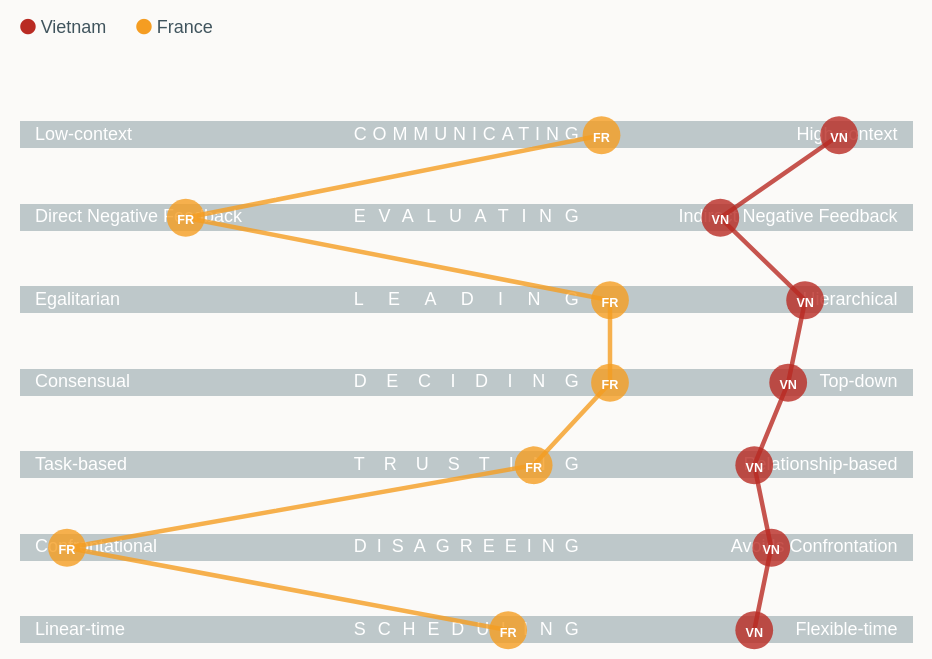
\includegraphics[width=3.11in,height=0.7\textheight]{figures/Culture_map_FR_VN.png}

}

\caption{Vietnam vs France across 7 dimensions introduced in The Culture
Map book\\
data source: \url{https://erinmeyer.com/tools/culture-map-premium}}

\end{figure}%

\begin{textblock}{2}(12,-4.5)
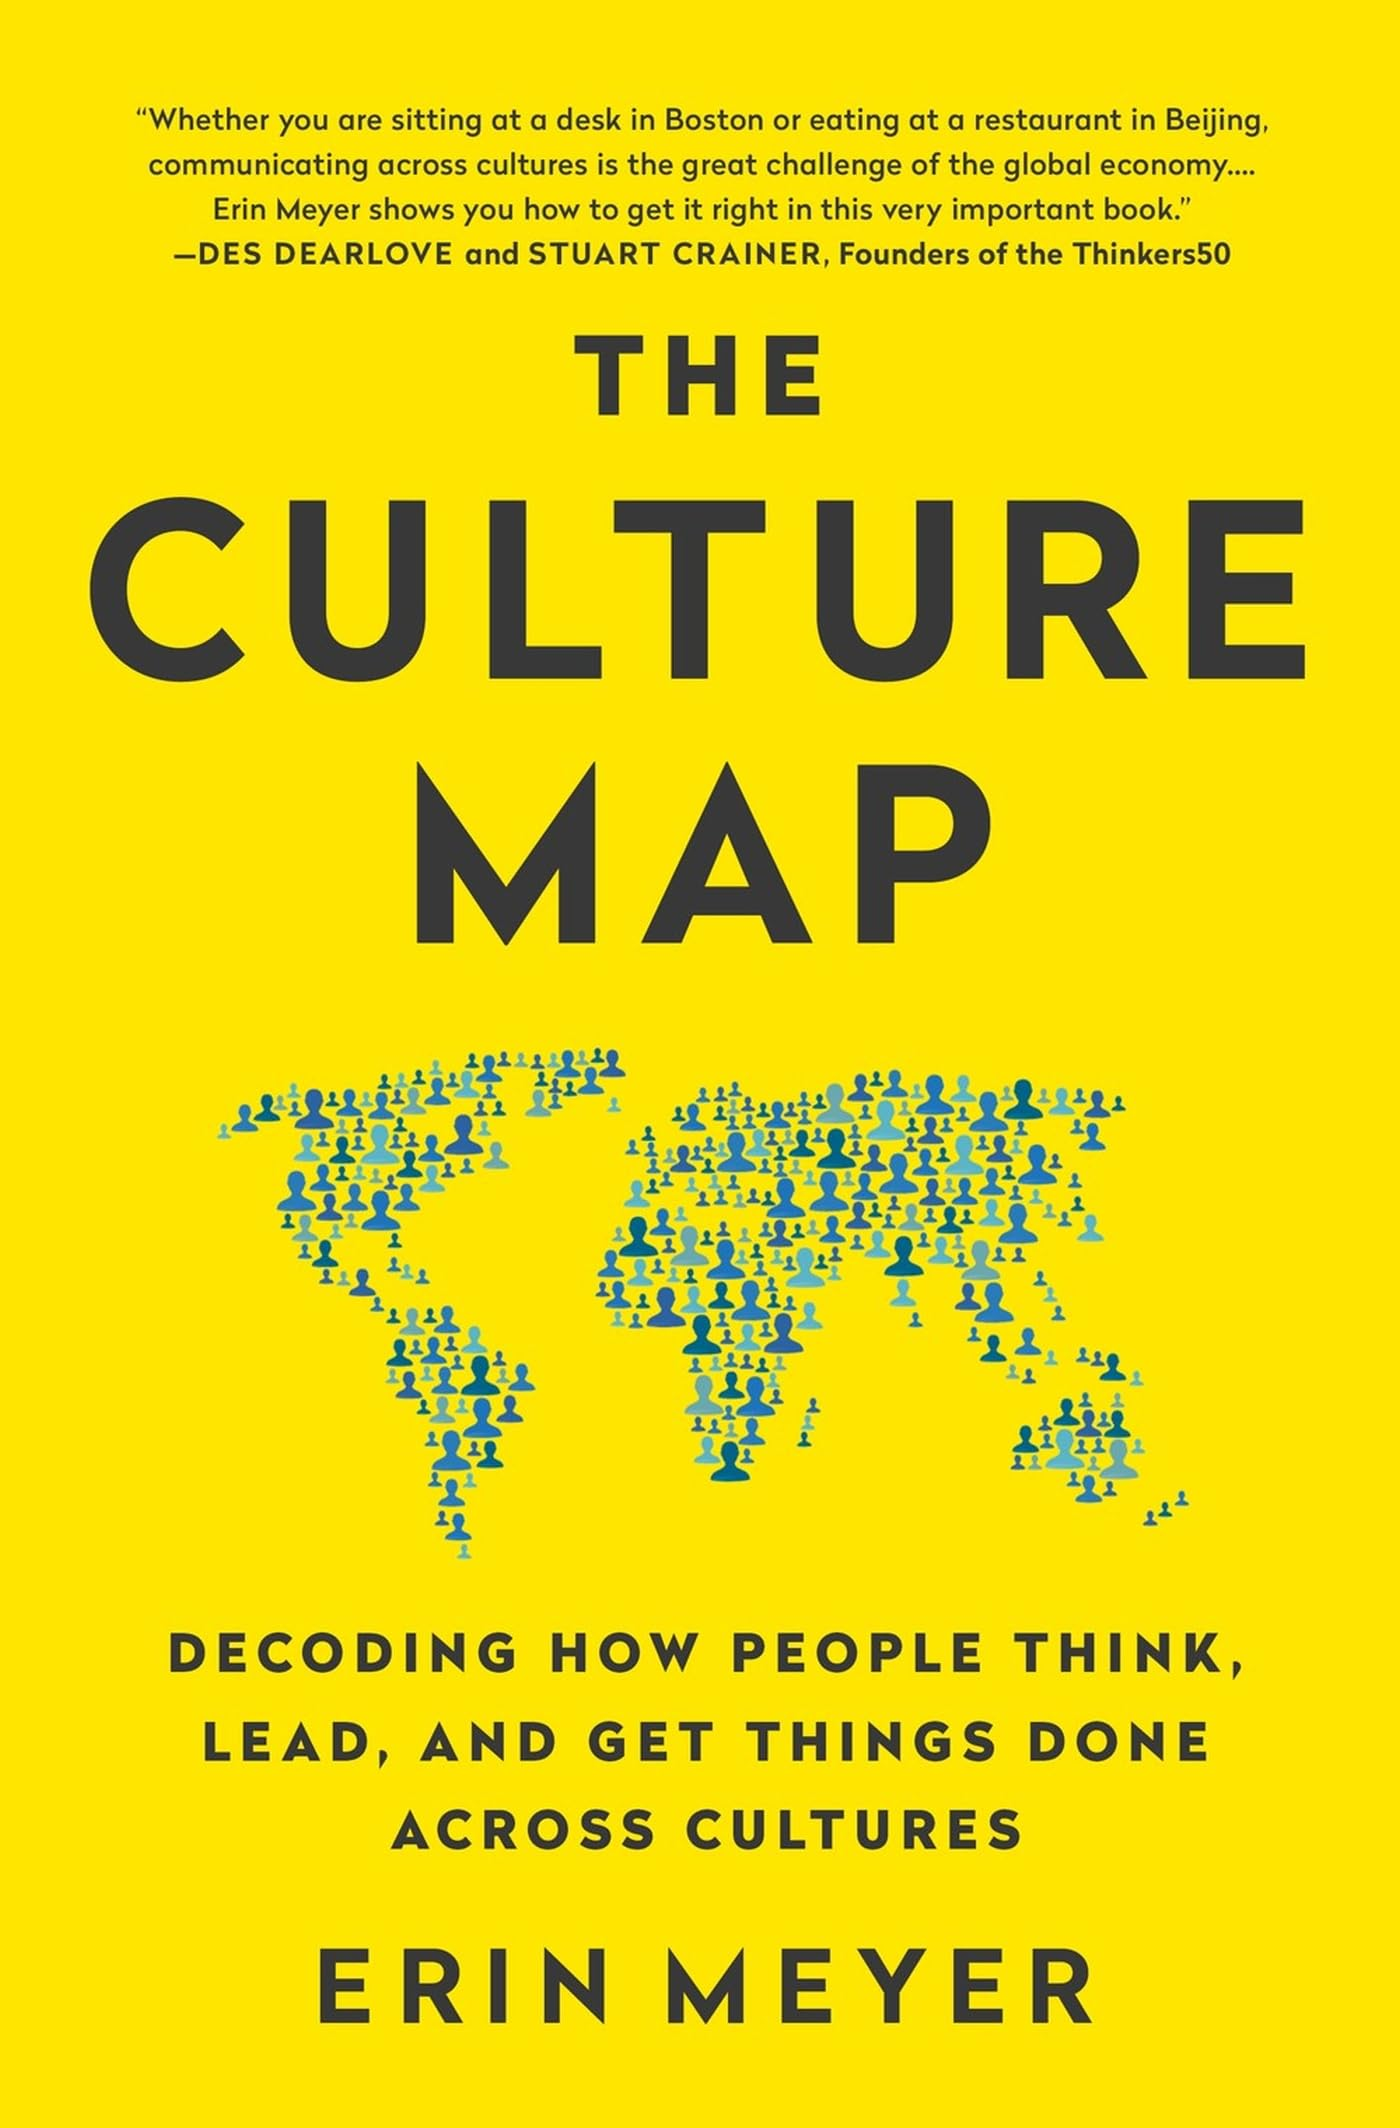
\includegraphics[width=2cm]{figures/Culture_map_bookcover.jpg}
\end{textblock}
\end{frame}

\section{What next?}\label{what-next}

\begin{frame}{Tentative schedule}
\protect\phantomsection\label{tentative-schedule}
{\def\LTcaptype{none} % do not increment counter
\begin{longtable}[]{@{}
  >{\raggedright\arraybackslash}p{(\linewidth - 6\tabcolsep) * \real{0.1029}}
  >{\raggedright\arraybackslash}p{(\linewidth - 6\tabcolsep) * \real{0.1471}}
  >{\raggedright\arraybackslash}p{(\linewidth - 6\tabcolsep) * \real{0.5294}}
  >{\raggedright\arraybackslash}p{(\linewidth - 6\tabcolsep) * \real{0.2206}}@{}}
\toprule\noalign{}
\begin{minipage}[b]{\linewidth}\raggedright
Day
\end{minipage} & \begin{minipage}[b]{\linewidth}\raggedright
Date
\end{minipage} & \begin{minipage}[b]{\linewidth}\raggedright
Morning
\end{minipage} & \begin{minipage}[b]{\linewidth}\raggedright
Afternoon
\end{minipage} \\
\midrule\noalign{}
\endhead
Day 1 & Aug.~24 & Introduction + R language & R language \\
Day 2 & Aug.~25 & Reproducible reporting + Practice & Core concepts \\
Day 3 & Aug.~26 & Core concepts & Linear Models \\
Day 4 & Aug.~27 & Linear Models & Linear Models \\
\bottomrule\noalign{}
\end{longtable}
}
\end{frame}

\section*{Questions?}\label{questions}




\end{document}
